As we stated in C.3, an experiment is designed to justify the positive impact of advanced TLBs. We compared two TLB shootdown granularities - per TLB entry v.s. whole TLB when the GPU page table is updated. The default implementation is to invalidate the whole TLB of every CU. Alternatively, only one TLB entry will be modified with TLB coherence. Although TLB coherence requires additional hardware support, it should have similar behavior with per TLB entry shootdown in terms of TLB hit rate.


As expected, smaller shootdown granularity gives higher hit rate because it keeps as much as valid translation information at any given time. The average hit rate difference is 11%.
However, TLB shootdown granularity has little effect on simulation cycles. This result demonstrates that if there is no significant latency improvement, the GPU barely benefit from TLB coherence model.

    \begin{figure}[!htb]
      \centering
      \setlength{\abovecaptionskip}{6pt plus 1pt minus 1pt}
      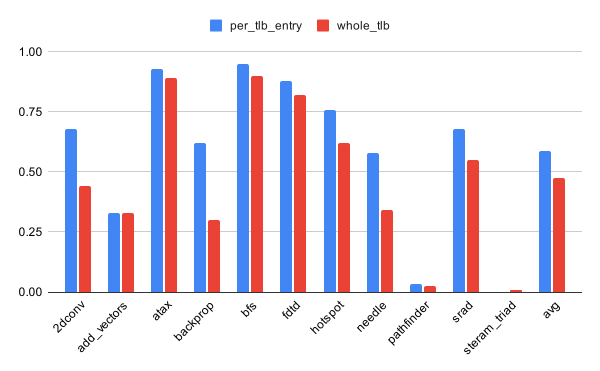
\includegraphics[width=.90\textwidth,keepaspectratio]{figures1/tlb_hit_rate.elf}
      \captionsetup{width=.75\textwidth}
      \caption{TLB hit rate for per TLB entry shootdown and whole TLB shootdown.}
      \label{fig:tlb_hr}
   \end{figure}

   \begin{figure}[!htb]
      \centering
      \setlength{\abovecaptionskip}{6pt plus 1pt minus 1pt}
      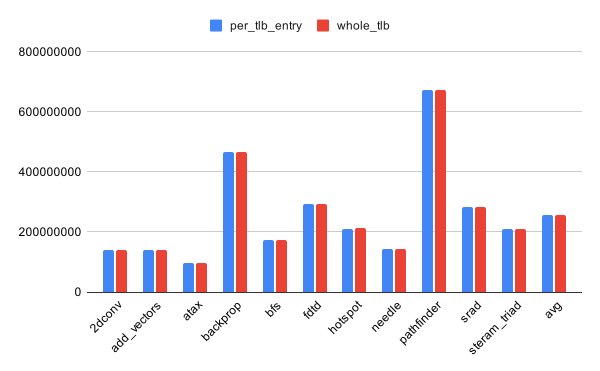
\includegraphics[width=.90\textwidth,keepaspectratio]{figures1/tlb_cycles.elf}
      \captionsetup{width=.75\textwidth}
      \caption{Simulation cycles for per TLB entry shootdown and whole TLB shootdown.}
      \label{fig:tlb_cycles}
   \end{figure}
